\chapter{Entwicklungsumgebung}

Für das Projekt sollte eine \acf{CI/CD} Pipline angelegt werden. Zu diesem Zweck wird ein Build Server in einer \acf{VM} gestartet. Der Code soll in einer Versionsverwaltung eingecheckt werden, um Änderungen nachvollziehbar zu machen und die Zusammenarbeit am Code zu vereinfachen.

\section{Werkzeuge und Anwendungen}

Der Code des projektes wird mit der Versionsverwaltungssoftware Git gemanagt (mehr zur Git Strategie in \autoref{chap:git-strat}). Um das Remote-Repository zu managen wird Github als Frontend eingesetzt (\url{https://Github.com/nilsrobinet/VertiefungSoftwareengineering}). Die \ac{CI/CD} Pipeline wird durch den quelloffenen Build-Server Jenkins gemanaged. Die Build-Toolchain wird in einem Docker-Container bereit gestellt. Der Build-Server läuft in einer \ac{VM}. Als Virtualisierungslösung wurde QEMU/KVM ausgewählt. Die Builds werden mittels CMake und Bash-Scipten konfiguriert. Für Erklärungen zu den verwendeten Werkzeugen siehe autoref{chap:tools}).

\section{Build-Server Setup}

Als Guest-Beriebsystem wurde sich für Arch Linux entschieden, da von diesem Betriebsystem bereits fertig vorgebaute \ac{VM} images bereit gestellt werden (\url{https://Gitlab.archlinux.org/archlinux/arch-boxes/-/packages}). Unter anderem wird ein qcow2 image das in der Virtualisierungsumgebung QEMU eingesetzt werden kann bereitgestellt.
In der \ac{VM} wird ein Jenkins build server installiert, der die \ac{CI/CD} Pipline bedient.

\subsection{Installation}

Die Build-Server \ac{VM} wurde auf ein Arch Linux System erstellt, einzelne Schritte, vor allem, wenn eine Paketverwaltungssoftware eingesetzt wird, können sich zwischen den verschiedenen Betriebsystemen unterscheiden.
Zur Erstellung und Installation wurden unter Arch Linux folgende Schritte durch geführt:

\begin{enumerate}
    \item Datenträgerabbild herunter laden:\\
        \lstinline[language=sh]!wget -O build_server.qcow2 https://Gitlab.archlinux.org/archlinux/arch-boxes/-/package_files/6852/download!
    \item Virtuelle Machine Starten:\\
    \lstinline[language=sh]!qemu-system-x86_64 -m 4G -smp 4 -enable-kvm\! \\
    \lstinline[language=sh]!                   -nic user,hostfwd=tcp::60022-:22,hostfwd=tcp::8090-:8090\ !\\
    \lstinline[language=sh]!                   build_server.qcow2!\\
    Der Benutzername und das Standartpasswort lauten: arch/arch; Man kann sich nun mittels ssh mit der \ac{VM} verbinden:\\
    \lstinline[language=sh]!ssh arch@localhost -p 60022!\\
    \item Jenkins installieren:\\
    \lstinline[language=sh]!pacman -Syu !\\
    \lstinline[language=sh]!pacman -S fontconfig!\\
    \lstinline[language=sh]!pacman -S freetype2!\\
    \lstinline[language=sh]!pacman -S jenkins!\\
    \lstinline[language=sh]!pacman -S docker!\\
    \lstinline[language=sh]!pacman -S Git!\\
    \lstinline[language=sh]!systemctl enable jenkins!\\
    \lstinline[language=sh]!systemctl enable docker!\\
    \lstinline[language=sh]!systemctl start jenkins!\\
    \lstinline[language=sh]!systemctl start docker!\\
    \lstinline[language=sh]!sudo usermod -aG docker jenkins!\\
    \item Nach der Installation kann über den Webrowser auf dem Host Beriebsystem unter der Addresse http://localhost:8090 auf die Jenkins Installation zugegriffen werden. Im initialen Setup-Dialog muss ausgewählt werden, ob die Standard-Plugins installiert werden sollen. Hier sollte mit ja geantwortet werden, und ein Admin Benutzer angelegt werden. Danach landet man im Haupmenu der Jenkins installation.

Zusätzlich wird noch das Plugin \glqq Docker Pipeline\grqq{} benötigt, das es ermöglicht in Docker-Images zu bauen. Diese lässt sich im Jenkins Plugin Manager installieren, der unter dem Menüpunkt \glqq Manage Jenkins \grqq{} zu finden ist.
\end{enumerate}

\subsection{Projekt einrichtung}

Unter dem Punkt \glqq new job\grqq{} wird ein neuer Multibranch Pipeline Job angelegt und konfiguriert.

\begin{figure}[H]
    \centering
    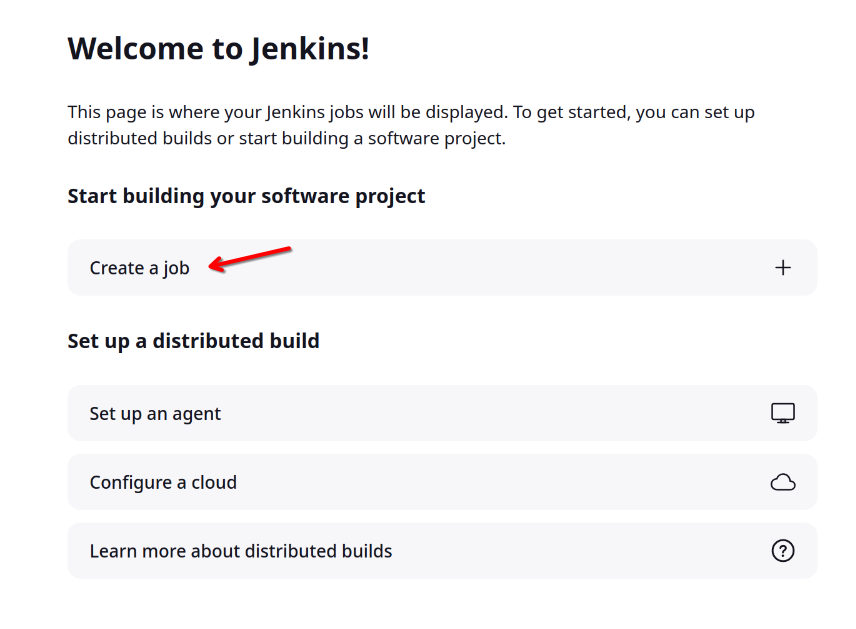
\includegraphics[scale=0.4]{res/Jenkins_01.png}
    \caption{Jenkins job erstellen.}
\end{figure}
\begin{figure}[H]
    \centering
    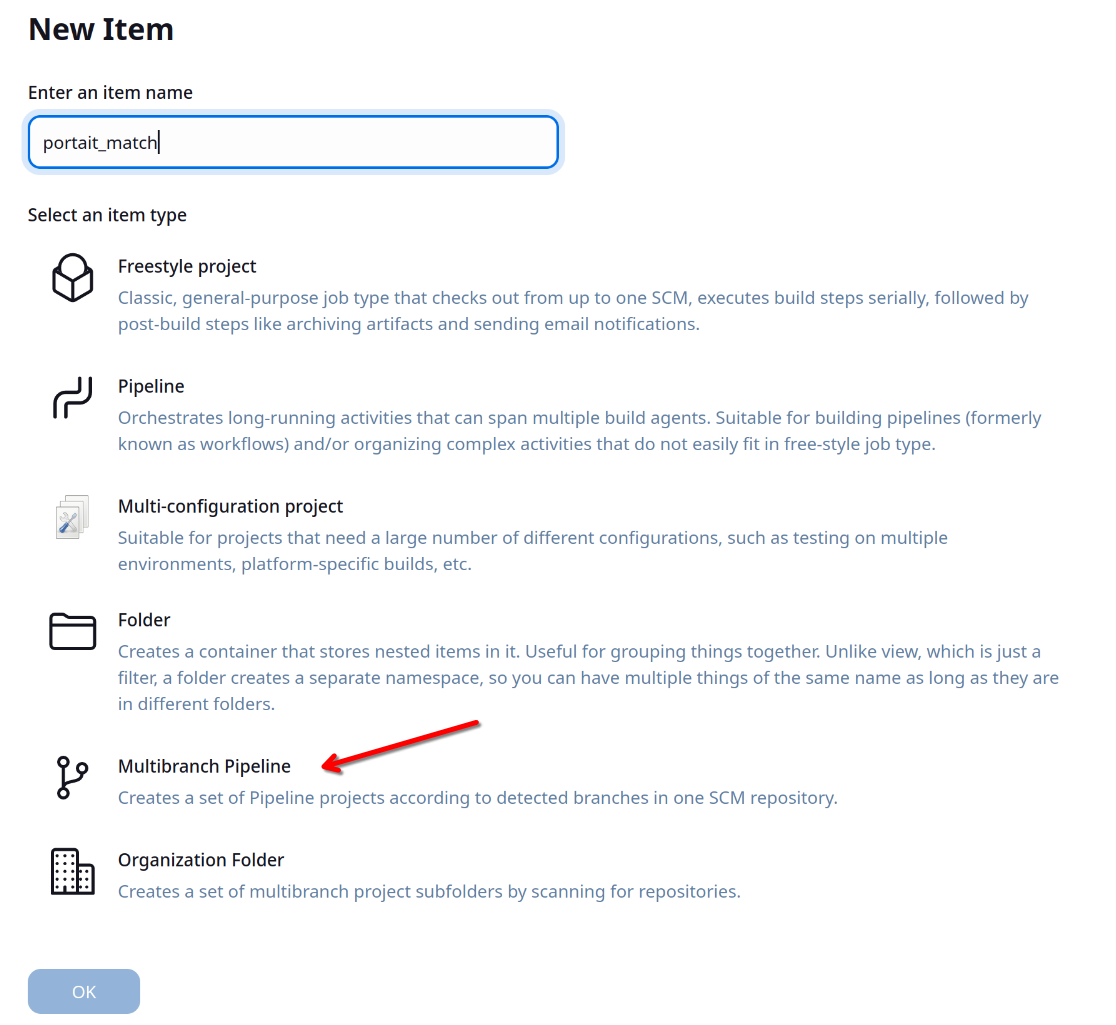
\includegraphics[scale=0.4]{res/Jenkins_02.png}
    \caption{Mutibranch Pipeline auswählen.}
\end{figure}
%\begin{figure}
%    \includegraphics[scale=0.25]{res/}
%    \caption{}
%\end{figure}

Als Branch Source wird das Github Repo dieses Projekts angegeben. Damit Jenkins auf das Projekt zu greifen kann, müsen noch Github Credentials eingratragen werden.

\begin{figure}[H]
    \centering
    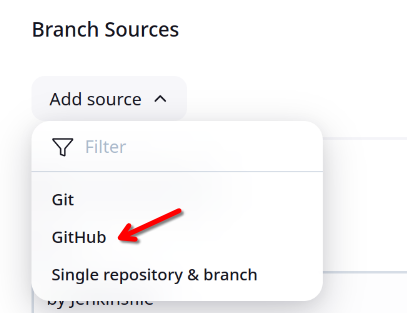
\includegraphics[scale=0.4]{res/Jenkins_03.png}
    \caption{Branch Source Auswahl.}
\end{figure}
\begin{figure}[H]
    \centering
    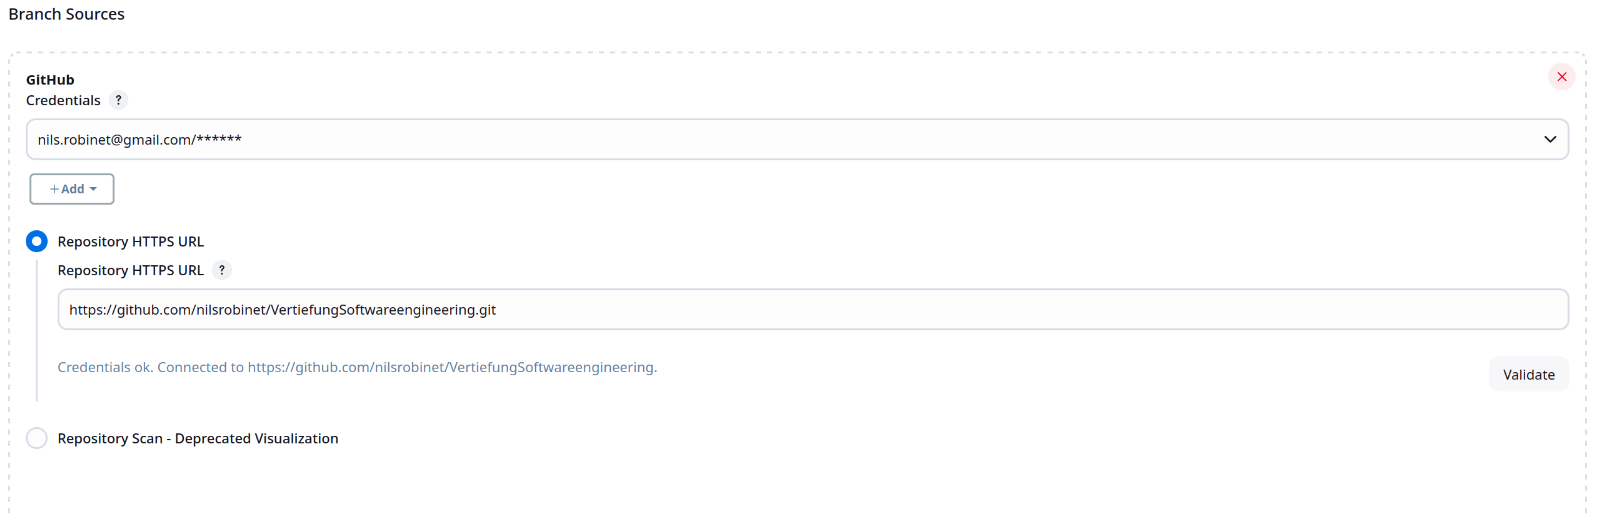
\includegraphics[scale=0.4]{res/Jenkins_05.png}
    \caption{Einstellung der Branch Source.}
\end{figure}

Damit Jenkins Änderungen zeitnah erkennt, wird ein periodischer Trigger mit einem Intervall von einer Minute eingestellt.

\begin{figure}[H]
    \centering
    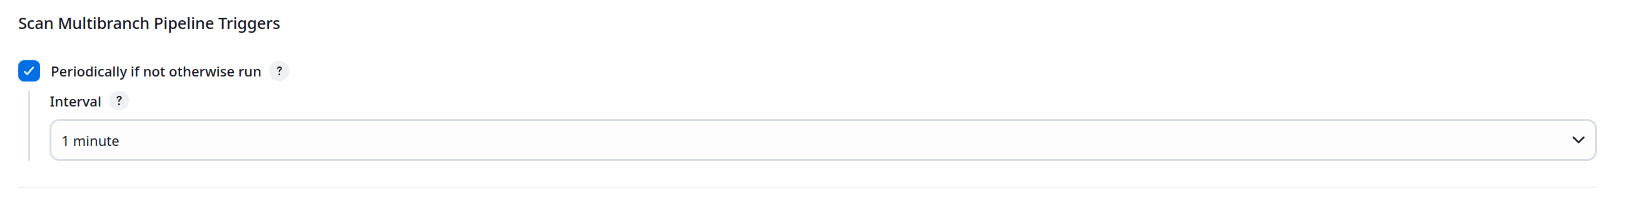
\includegraphics[scale=0.4]{res/Jenkins_06.png}
    \caption{Einstellung des Repository Polling Intervalls.}
\end{figure}

Danach ist das Projekt fertig konfiguriert und kann benutzt werden.

Die Build und Deployment stages werden durch das im Repositroy eingecheckte Jenkinsfile konfiguriert. Der Build findet in einem Docker-Container statt, der durch ein Dockerfile, das ebenfalls eingecheckt ist, erstellt wird. Das Docker-Image wird durch Jenkins gemanagt. Jenkins kümmert sich auch darum, das Docker-Image bei Änderungen am Dockerfile neu zu generieren.

\subsection{Pipeline Konfiguration}

Die Build-/Deployment-Pipeline wird durch die Datei Jenkisfile, die im Root-Verzeichnis des Projekts liegt, konfiguriert. Für jeden Branch kann dabei eine andere Konfiguration in der zugehörigen Jenkisfile Datei angelegt werden. Dadurch können Entwickler auf ihrem Branch ungestört neue Features, die Änderungen and der CI/CD-Pipeline nach sich ziehen, hoch bringen, ohne andere Branches wie den \glqq develop \grqq{} oder \glqq main \grqq{} Branch zu beeinflussen.
Im Unterordner \lstinline{build_scripts} liegen Skript-Dateien welche in den einzelnen Schritten der Pipeline aufgerufen werden. Mit Hilfe dieser Skripte werden dann die eigentlichen Builds und Deployments durchgeführt.

Jenkins wertet die Jenkinsfile Datei automatisch aus und führt die darin beschriebenen Schritte durch. Die Datei ist hirarchich aufgebaut. In der obersten Ebene wird durch den Key \glqq pipeline\grqq{} festgelegt, das eine Pipeline beschrieben werden soll. In der Ebene darunter wird unter dem Key \glqq agent\grqq{} festgelget, wo das Projekt gebaut werden soll und welche Voraussetzungen die Build-Agents mitbringen müssen. Da keine anderen Build agents angelegt wurden, wird das Projekt direkt auf dem Jenkins server gebaut. Aus diesem Grund wird an dieser Stelle nur festgelegt, dass das Projekt in einem Docker Container gebaut werden soll. Der Docker Container wird durch das Dockerfile, welches ebenfalls im Root-Verzeichniss des Projekts eingecheckt ist, erstellt. Da Jenkins nur das Dockerfile bekannt gemacht wurde, übernimmt Jenkins das Managemnt der Images. Das Bedeutet unter anderem, dass Jenkins automatisch detektiert ob sich das Dockerfile geändert hat und ob ein neues Image gebaut werden muss.


Unter dem Key \glqq stages\grqq{} werden die Einzelschritte der Pipeline fest gelegt. In diesem Fall sind das vier Schritte:
\begin{enumerate}
    \item{Build:} In der Build-Stage wird das Skript makeC.sh aufgerufen, das mit Hilfe des tools CMake (siehe \autoref{chap:tools}) die C++ und Cython Komponenten des Projekts baut und in das Verzeichnis bin installiert. Das Skript wird anstelle von Jenkins Boardmitteln verwendet, sodass lokal wie auf dem Buildserver das gleiche Skript genutzt werden kann um das Proekt zu bauen. Dadurch können sich die Iterationszeiten bei Änderungen am C++ Quellcode verringern, da Probleme, die beim Bauen auf dem Build-Server auftreten, einfach nachgestellt werden können.
    
    Außerdem wird in der Build-Stage das Skript makedemo.sh aufgerufen, mit welchem ein Docker-Container gebaut wird, der die Anwendung enthält, die in der Deployment-Stage ausgeliefert wird.
    \item{Test:} In dieser Stage werden verschiedene Tests mit den Tools ctest (C Unit tests) und pytest (Python tests) und pylint (Python Linting) ausgeführt. Die Ergbnisse werden im junit-xml Format gespeichert, damit sie später im \glqq post\grqq-Teil der Pipeline ausgewertet werden können.
    \item{Docu:} In dieser Stage wird die Dokumentation generiert. Dazu wird das Skript makedoc.sh genutzt, welches diese Ausarbeitung sowie die Doxygen-Dokumentation der C++ Komponenten generiert.
    \item{Deploy:} In dieser Stage wird das fertig kompilierte und installierte Programm ausgeliefert und gestartet. Hierzu wird das Skript deploy.sh verwendet.
    In der Deployment-Stage wird eine \glqq when\grqq{} Bedingung eingesetzt, um zu verhindern, dass andere Branches als der \glqq main\grqq-Branch in das Produktiv-System deployt werden.
\end{enumerate}

Der Key \glqq post\grqq{} beschreibt was nach dem Build und Deploy geschehen soll. Dazu gehört das Speichern von artifakten, die behalten werden sollen und das Auswerten von Testergebnissen.

\begin{figure}
    \label{fig:test_results}
    \centering
    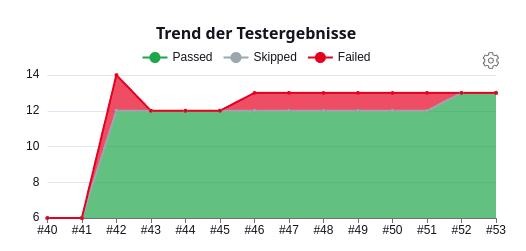
\includegraphics[scale=0.4]{res/Jenkins_test_results.png}
    \caption{Testergbnisse der letzten Builds auf einem Feature-Branch nachdem die Auswertung der junit-xml Ergbinise aktiviert wurde.}
\end{figure}

\lstinputlisting[language=json]{../../Jenkinsfile}

\subsection{Buildumgebung}
Die Buildumgebung wird in einem Docker Container bereitgestellt. Das Docker Image wird durch ein Dockerfile erzeugt:

\lstinputlisting[language=bash]{../../Dockerfile}

Das Image basiert auf einem Ubuntu Image, in das zusätzlich alle Tools installiert werden, die im Buildprozess benötigt werden.

Die Skripte die zum Bauen verwendet werden befinden sich im Verzeichnis \glqq build\_scripts\grqq{}. In diesem Verzeichnis liegen auch Skripte die das lokale Arbeiten vereinfachen sollen: Unter Anderem liegen hier Skripte, die das Bauen des Dockerimages automatisieren und ein Skipt, das den Container interaktiv startet und das Repository mountet.

Der Build an sich wird mittels CMake konfiguriert und mit Make durchgeführt. Als Kompiler für die C++ Quelldateien wird auf gcc gesetzt (siehe \autoref{chap:tools}). Als C++ Standart wird C++20 eingesetzt und der Kompiliervorgang wird mit den folgenden Flags eingestellt: \lstinline{-O3 -Wall -Werror -Wno-strict-aliasing}. Das Flag O3 bedeutet, dass mit der höchsten Optimierungsstufe gebaut werden soll. Wall heißt, dass der Kompiler alle Warnungen ausgeben soll und Werror bedeutet, dass Warnungen als Fehler behandelt werden sollen und der Build abbrechen soll, wenn eine Warnung auftritt. Mit Wno-strict-aliasing wird die strict-aliasing warnung ausgeschaltet, die einige Pointer casts verhindert. Das ist notwendig, da für die Entwicklung einer C++ Bibliothek mit Python kompatiblen Interface Pointer aus dem Speicherbereich des Python-Interpreters manipuliert werden müssen.

\subsection{Deployment}

Das Deployment wird mit Hilfe des Skripts deploy.sh ausgeführt.

\lstinputlisting[language=bash]{../../build_scripts/deploy.sh}

Mit Hilfe des Datei-Kopierwerkzeugs \glqq rsync\grqq{} wird das Docker-Image, das in der Build-Stage gebaut wurde auf den Zielserver kopiert. Dann wird über SSH auf den Zielserver zugegriffen und das Kopierte Docker-Image geladen und gestartet. Das Docker-Image enthält die Demoanwendung und führt diese beim Start aus.
